\setcounter{section}{3}
\section{Implement Policy Gradient}
\subsection{\texttt{CartPole-v0}}
The learning curves for the small and large batch experiments on the
\texttt{CartPole-v0} environment are show in \figref{small-cartpole} and
\figref{large-cartpole}.

\begin{itemize}
  \item
    For both small and large batches, the gradient estimator using reward-to-go
    has higher average return and less variance than the gradient
    trajectory-centric estimator.

  \item
    The performance of the reward-to-go gradient estimator with and without
    advantage normalization is comparable. For both the small and large batch
    experiments, the average returns are similar. There are slight differences,
    but it's hard to tease out what is caused by noise and what is caused by
    the advantage normalization.

  \item
    The derivation of the trajectory-based gradient estimator is very rigorous,
    and the derivation of the reward-to-go gradient estimator is a bit more
    ``hand-wavy''. Empirically (and intuitively, the reward-to-go estimator
    performs better. Moreover, advantage normalization should help in theory,
    but in practice seems underwhelming.

  \item
    The larger batch size helps a lot. The average return saturates at 200 with
    fewer iterations, and the variance is much smaller.

  \item
    The script used to run the \texttt{CartPole-v0} experiments is given in
    \figref{cartpole-script}.
\end{itemize}

\subsection{\texttt{InvertedPendulum-v1}}
The learning curve for the \texttt{InvertedPendulum-v1} environment is given in
\figref{pendulum}. The script used to run the experiments is given in
\figref{pendulum-script}. I used a rather normal learning rate (0.01), pretty
standard network architecture (2 hidden layers with 32 units each), and a
reasonably large batch size (10,000). The large batch size greatly helped
reduce the variance and increase average return. Smaller batch sizes would
sometimes obtain a score of 1000, but would fluctuate wildly.

\begin{figure}[h]
  \centering
  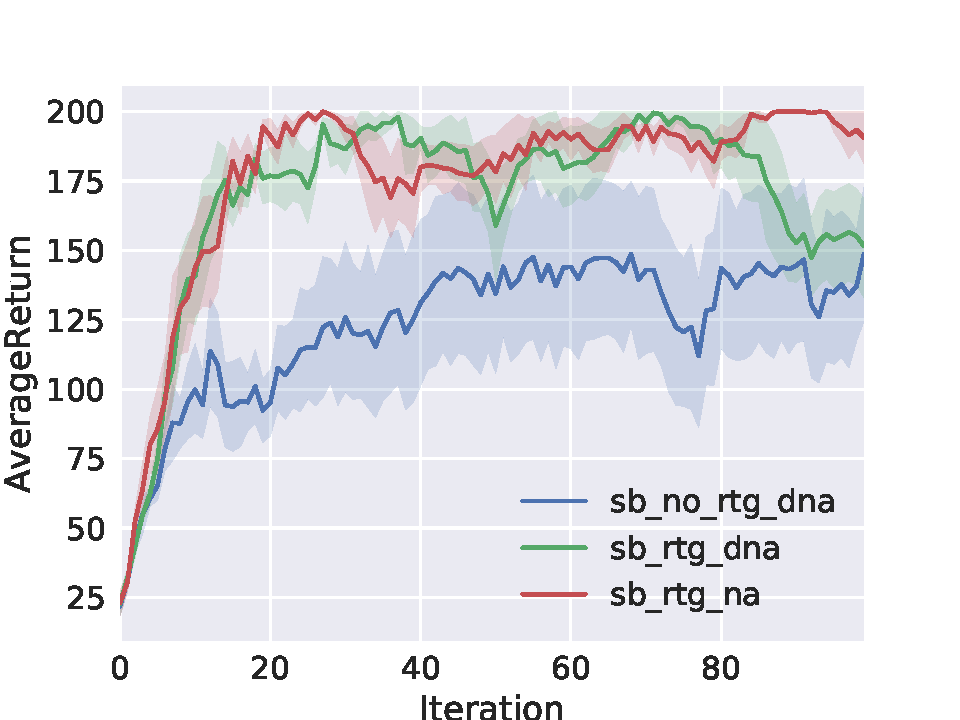
\includegraphics[width=0.8\textwidth]{cartpole_small.pdf}
  \caption{%
    Learning curves (average return at each iteration) for
    the \texttt{sb\_no\_rtg\_dna}, \texttt{sb\_rtg\_dna}, and
    \texttt{sb\_rtg\_na} experiments run on the \texttt{CartPole-v0}
    environment.
  }
  \label{fig:small-cartpole}
\end{figure}

\begin{figure}[h]
  \centering
  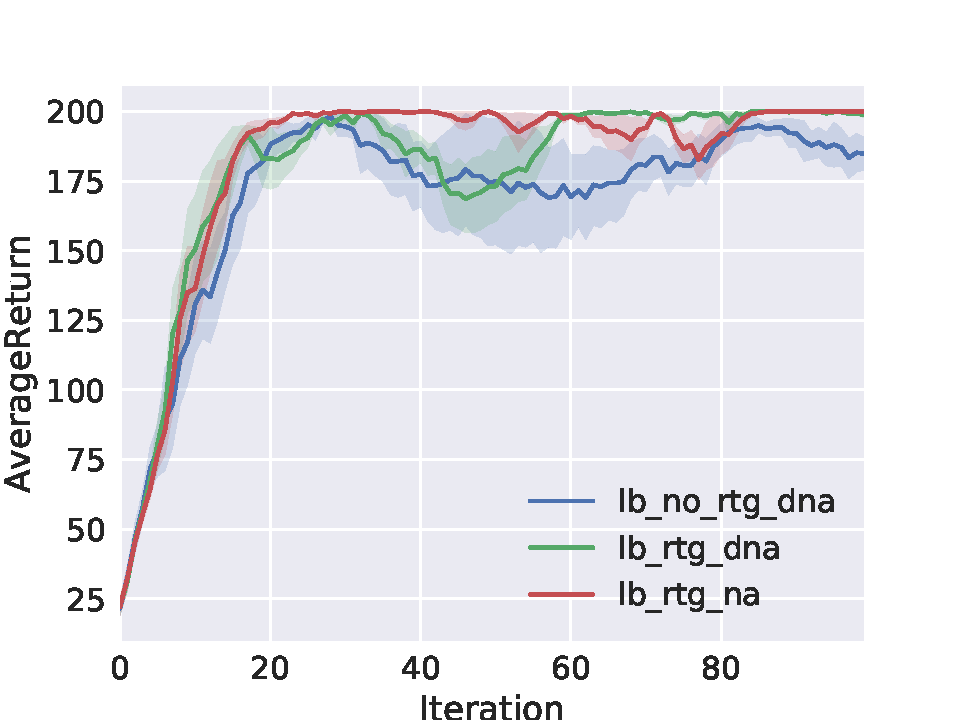
\includegraphics[width=0.8\textwidth]{cartpole_large.pdf}
  \caption{%
    Learning curves (average return at each iteration) for
    the \texttt{lb\_no\_rtg\_dna}, \texttt{lb\_rtg\_dna}, and
    \texttt{lb\_rtg\_na} experiments run on the \texttt{CartPole-v0}
    environment.
  }
  \label{fig:large-cartpole}
\end{figure}

\begin{figure}
  \centering
  \scriptsize
  \begin{Verbatim}[gobble=4]
    #! /usr/bin/env bash

    set -euo pipefail

    main() {
        n=100
        e=5
        flags="--verbose --n_layers 1 --size 32"
        set -x
        python train_pg.py CartPole-v0 $flags -n $n -b 1000 -e $e      -dna --exp_name sb_no_rtg_dna
        python train_pg.py CartPole-v0 $flags -n $n -b 1000 -e $e -rtg -dna --exp_name sb_rtg_dna
        python train_pg.py CartPole-v0 $flags -n $n -b 1000 -e $e -rtg      --exp_name sb_rtg_na
        python train_pg.py CartPole-v0 $flags -n $n -b 5000 -e $e      -dna --exp_name lb_no_rtg_dna
        python train_pg.py CartPole-v0 $flags -n $n -b 5000 -e $e -rtg -dna --exp_name lb_rtg_dna
        python train_pg.py CartPole-v0 $flags -n $n -b 5000 -e $e -rtg      --exp_name lb_rtg_na
        set +x
    }

    main
  \end{Verbatim}
  \caption{Script use to run \texttt{CartPole-v0} experiments.}
  \label{fig:cartpole-script}
\end{figure}

\begin{figure}[h]
  \centering
  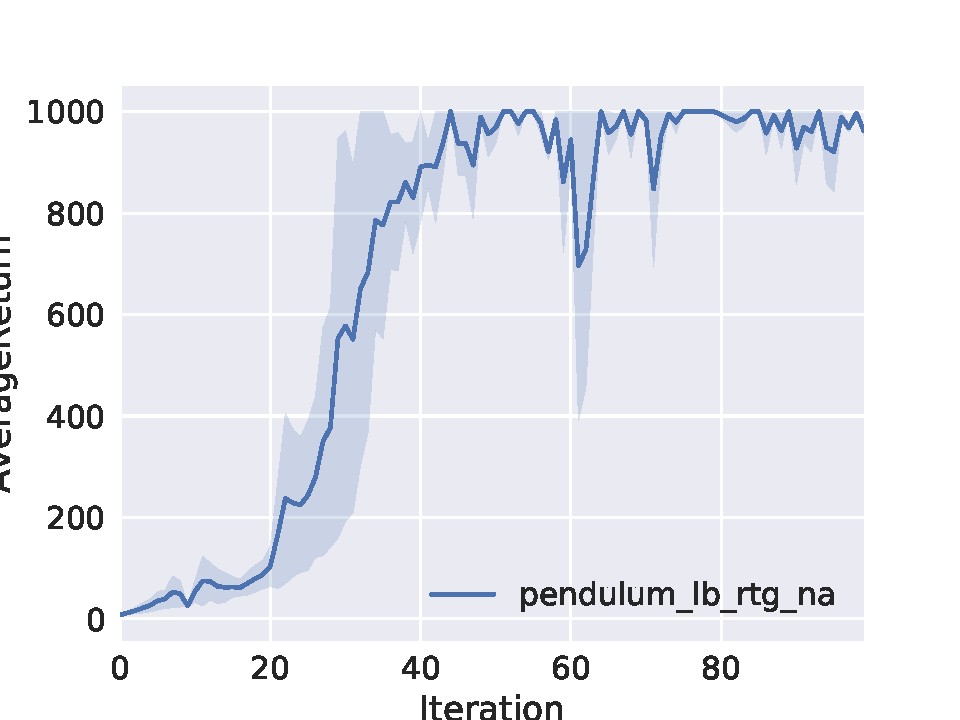
\includegraphics[width=0.8\textwidth]{pendulum.pdf}
  \caption{%
    A learning curve for a policy which obtains an average return of 1000 in
    fewer than 100 iterations. A batch size of 10,000 was used.
  }
  \label{fig:pendulum}
\end{figure}

\begin{figure}
  \centering
  \footnotesize
  \begin{Verbatim}[gobble=4]
    #! /usr/bin/env bash

    set -euo pipefail

    main() {
        python train_pg.py \
            InvertedPendulum-v1 \
            --verbose \
            --n_layers 2 \
            --size 32 \
            --seed 2 \
            -n 100 \
            -b 10000 \
            -e 2 \
            --discount 1 \
            --learning_rate 0.01 \
            -rtg \
            --exp_name pendulum_lb_rtg_na
    }

    main
  \end{Verbatim}
  \caption{Script use to run \texttt{InvertedPendulum-v1} experiments.}
  \label{fig:pendulum-script}
\end{figure}
